%%%%%%%%%%%%%%%%%%%%%%%%%%%%%%%%%%%%%%%%%%%%%%%%%%%%%%%%%%%%%%%%%%%%%%%%%%%%%%%%
% mini-MQ: learning-scale distributed message queue --- paper (USENIX style)
%
% Compile: pdflatex paper && bibtex paper && pdflatex paper && pdflatex paper
%
% All performance numbers in this paper are regenerable from committed
% evidence files; see the Availability section and paper/make-figures.py.
%%%%%%%%%%%%%%%%%%%%%%%%%%%%%%%%%%%%%%%%%%%%%%%%%%%%%%%%%%%%%%%%%%%%%%%%%%%%%%%%

\documentclass[letterpaper,twocolumn,10pt]{article}
\usepackage{usenix2019_v3}

\usepackage{tikz}
\usetikzlibrary{positioning,arrows.meta}
\usepackage{amsmath}
\usepackage{booktabs}

% small muted note text used inside TikZ nodes
\newcommand{\fnote}[1]{{\scriptsize\color{black!60}#1}}

%-------------------------------------------------------------------------------
\begin{document}
%-------------------------------------------------------------------------------

\date{}

\title{\Large \bf mini-MQ: A Learning-Scale Distributed Message Queue with
  Chaos-Verified Durability and Honest Benchmarks}

\author{
{\rm Jianhua Guo}\\
Shenzhen University\\
1125448766@qq.com
}

\maketitle

%-------------------------------------------------------------------------------
\begin{abstract}
%-------------------------------------------------------------------------------
Log-based message queues such as Kafka, RocketMQ, and Pulsar are critical
infrastructure, yet their size makes their load-bearing mechanisms hard to
study as executable systems. We present \textbf{mini-MQ}, a distributed
message queue of ${\sim}16.7$k lines of Java that reproduces those mechanisms
with industrial fidelity: a RocketMQ-style single CommitLog with sparse
consume indexes and CRC-based crash recovery; a 16-byte framed binary
protocol; a two-parameter group-commit flush that raises forced-fsync
throughput from 83 to 714{,}285\,msg/s; Kafka-style pull replication with
leader-epoch arbitration and high watermarks; and a Raft-style election
kernel with PreVote. Durability is not asserted but \emph{chaos-verified}:
a 12-cell fault matrix with deterministic injection hooks kills, partitions,
and resurrects leaders under load and hard-asserts RPO~$=0$ per cell under
\texttt{acks=all}, with worst-case recovery (RTO) of 2.9\,s. We benchmark
honestly against Kafka 4.1.2 on the same host---51\% of its throughput and
1.65$\times$ its P99 latency---and attribute the gap to four profiled
mechanisms, explicitly declaring the share we cannot yet explain. Every
number in this paper regenerates from committed evidence files by script.

\end{abstract}

%-------------------------------------------------------------------------------
\section{Introduction}
%-------------------------------------------------------------------------------

Distributed message queues are the connective tissue of modern data
infrastructure: they decouple producers from consumers, absorb load spikes,
and act as the durable commit log around which streaming architectures are
built~\cite{kreps13log,kleppmann17ddia}. Their designs encode decades of
hard-won mechanism knowledge---sequential-write storage layouts,
pull-based replication, quorum-managed in-sync replica sets, group-commit
fsync amortization, zero-copy delivery. Yet precisely because these systems
are production hardened, they are difficult to learn from directly: the
mechanisms sit buried inside hundreds of thousands of lines of mature code,
and textbook descriptions diverge from the code that actually runs.

This paper describes \textbf{mini-MQ}, a message queue built to make those
mechanisms \emph{executable} at a scale a single engineer can hold in their
head. The goal is not to compete with Kafka on features; the goal is
industrial \emph{fidelity of the core} with pedagogical \emph{size}: five
core modules totaling ${\sim}16.7$k lines of Java
(storage~3.4k, protocol~0.7k, replication~2.7k, broker~4.2k,
client~5.6k), plus a 2.5k-line benchmark harness. Three commitments
distinguish mini-MQ from a typical course project:

\begin{description}
\item[Real processes, real faults.] A cluster is three real JVMs. Leaders
  are killed with \texttt{SIGKILL} mid-write-storm; the network is split
  bidirectionally and unidirectionally with a TCP proxy shield; a stale
  leader is resurrected to fight for its old position. Every failure cell
  ends with a hard reconciliation: \emph{acked messages read back exactly,
  or the test fails}.
\item[Deterministic chaos.] Faults fire at \emph{named program moments}---
  during an election, inside a flush window, inside a write storm---using
  atomic-counter time-point hooks, so rerunning one command reproduces the
  same fault at the same moment (\S\ref{sec:chaos}).
\item[Honest measurement.] Every claim in this paper traces to a committed
  evidence file, and the comparison against Kafka reports the numbers we
  \emph{lost}: 51\% of Kafka's throughput and 1.65$\times$ its P99, with the
  gap attributed bucket-by-bucket to profiled mechanisms and the
  unexplained remainder explicitly declared rather than
  hidden~(\S\ref{sec:eval-kafka}).
\end{description}

\noindent
This last commitment deserves a word of motivation. Small-system writeups
tend to report green dashboards: tests pass, the demo works. We instead
treat \emph{measurement honesty} as a first-class artifact, on the argument
that a learning-scale system's credibility comes from verified invariants
(what is asserted, under injected faults, per cell) and from calibrated
expectations (what the system demonstrably is, relative to the industry
reference on the same hardware). Concretely, mini-MQ's reliability claims
are backed by a 12-cell chaos matrix with per-cell RPO assertions, and its
performance claims are backed by same-host Kafka runs whose parameters were
aligned along seven dimensions---with every asymmetry that remained (round
length, client batching) declared in the results table.

Our contributions:

\begin{itemize}
\item \textbf{A hybrid architecture at learning scale}
  (\S\ref{sec:arch}): RocketMQ's storage gene (single CommitLog, sparse
  ConsumeQueue), Kafka's replication gene (pull-based fetch, leader epochs,
  high watermarks, ISR with $\mathtt{min.insync.replicas}=2$ loud failure),
  and a Raft-style election kernel (terms, majority, PreVote)---the same
  control-plane/data-plane split that Kafka itself made in
  KRaft~\cite{kip500}.
\item \textbf{Chaos-verified durability} (\S\ref{sec:chaos}): a
  deterministic fault-injection toolkit and a 12-cell matrix asserting
  RPO~$=0$ under \texttt{acks=all} for leader/follower \texttt{kill -9}
  during elections, flush windows, and write storms; bidirectional and
  one-way partitions; stale-leader revival; ISR shrink; minority partition;
  and retry storms. Worst-case RTO is 2.9\,s against an 8\,s budget; the
  two \emph{loud} unavailability windows (18.3--23.7\,s and 4.4--4.7\,s)
  are reported separately rather than folded into RTO. The matrix found two
  real bugs before it turned green (\S\ref{sec:chaos-bugs}).
\item \textbf{Mechanism-level performance with profiled evidence}
  (\S\ref{sec:eval}): two-parameter group commit turning a 38{,}055$\times$
  fsync wall into an 11\% cost at 8 producers (records per fsync rising
  241$\rightarrow$909); profiling-driven optimization of the send-path
  lock critical section (2.4\%$\rightarrow$0.3\% of samples, +3.4\%
  throughput) and of hot-path allocations (stack-rental object pools,
  $-17.3\%$ sampled bytes); and a replication-loop race fix that took
  false ISR evictions from 5{,}308 per 60{,}000 writes to zero.
\item \textbf{An honest same-host comparison with Kafka 4.1.2}
  (\S\ref{sec:eval-kafka}): 38{,}001 vs.\ 74{,}776\,msg/s end-to-end
  (RF=3, \texttt{acks=all}, 1\,KiB), P99 1{,}555 vs.\ 943\,ms, with
  P50 parity (711 vs.\ 725\,ms)---attributed to four buckets with
  profiled evidence, and a declared unattributed remainder.
\end{itemize}

mini-MQ is fully open source; one script builds it, boots a three-node
cluster, reconciles a 10{,}000-message smoke run, and tears it down in
under ten minutes (\S\ref{sec:availability}).

%-------------------------------------------------------------------------------
\section{Background and Design Lineage}
%-------------------------------------------------------------------------------

\subsection{The log as the primitive}
An append-only, totally ordered log is the simplest durable structure that
supports both queueing and replay~\cite{kreps13log}. The engineering
questions are all in the margins: how to write it fast (sequential writes,
page cache, batching of \texttt{fsync}), how to replicate it safely
(quorums, epochs, watermarks), and how to find data in it afterwards
(indexes). Production systems answer these differently, and their answers
are the ``genes'' a learning-scale system must choose among.

\subsection{Three production genes}
\textbf{Kafka}~\cite{kreps11kafka,kafkadocs} keeps one partitioned log per
topic-partition and replicates by \emph{pull}: followers fetch byte ranges
from the leader, which fences stale leaders with \emph{leader epochs} and
publishes the committed prefix as a \emph{high watermark} (HW). Replication
membership is the ISR; writes with \texttt{acks=all} wait for the full ISR.
Since KRaft~\cite{kip500}, Kafka separates a Raft-based metadata quorum
(control plane) from the per-partition fetch data plane. \textbf{RocketMQ}%
~\cite{rocketmqdocs} instead appends \emph{all} topics to a single
per-broker CommitLog and builds sparse per-topic ConsumeQueue indexes by
replay, buying one sequential write stream at the cost of read
indirection. \textbf{Pulsar}~\cite{pulsardocs} segments every topic into
ledgers spread over BookKeeper bookies, decoupling storage from compute.

mini-MQ takes RocketMQ's storage gene (a single CommitLog per broker is the
cleanest sequential-write layout at three-node scale), Kafka's replication
gene (pull fetch, epochs, HW, ISR), and a Raft-style election kernel for
the control plane---the same hybrid Kafka arrived at with
KRaft~\cite{ongaro14raft,kip500}. Eight architecture decision records,
each with rejected alternatives and explicit invalidation boundaries,
document why~\cite{nygard11adr}; e.g., layered storage was rejected
because a three-node deployment cannot cash its benefits.

\subsection{The economics of durability}
\texttt{fsync} on a spinning or NVMe-backed filesystem serializes at
roughly one call per millisecond; a naive \emph{ack-after-every-fsync}
policy caps throughput at the fsync rate. Group commit---accumulate
concurrent writes, flush once, acknowledge all---is the classic answer in
databases~\cite{gray93tp}, shipped as \texttt{ordered\_commit()} in
MySQL's binlog~\cite{mysqlbinlog}. \S\ref{sec:eval-groupcommit} measures
this wall in mini-MQ (83\,msg/s per-record force) and the group-commit
curve that removes it.

%-------------------------------------------------------------------------------
\section{Architecture}
\label{sec:arch}
%-------------------------------------------------------------------------------

\begin{figure*}[t]
\centering
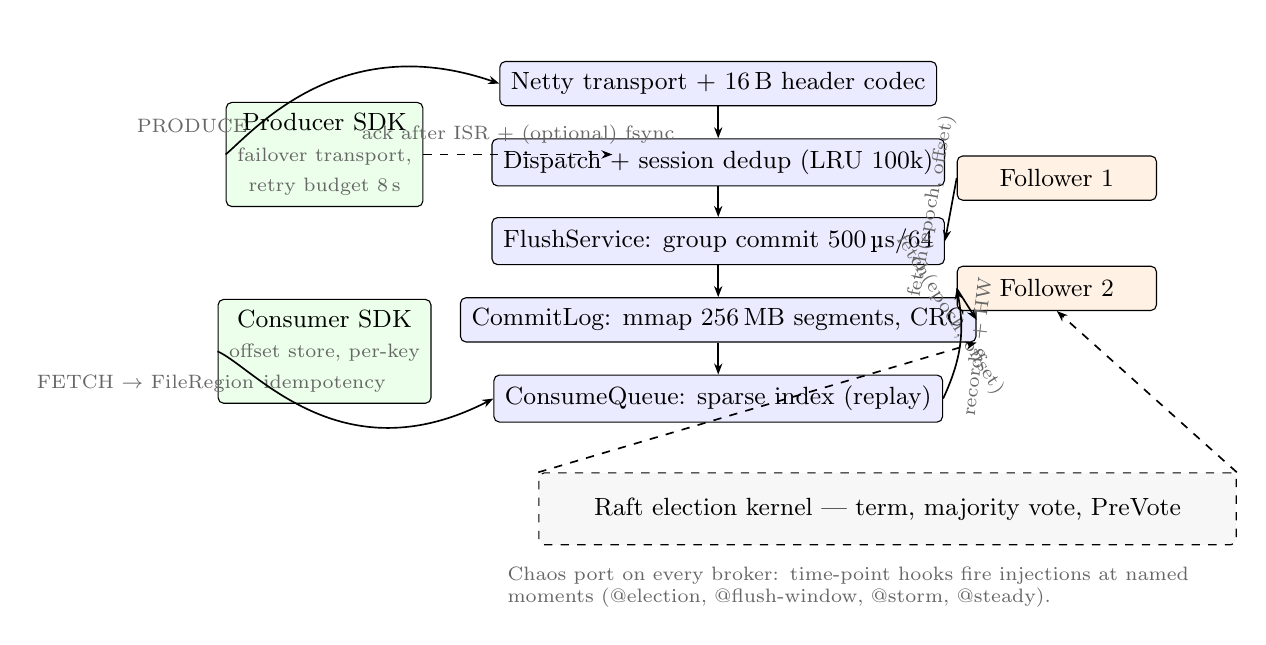
\begin{tikzpicture}[
  font=\small,
  box/.style={draw, rounded corners=2pt, align=center, inner sep=4pt,
              minimum height=16pt},
  mod/.style={box, fill=blue!8},
  cli/.style={box, fill=green!8},
  fol/.style={box, fill=orange!10, minimum width=72pt},
  arr/.style={-{Stealth[length=4pt]}, semithick},
  darr/.style={-{Stealth[length=4pt]}, semithick, dashed},
  note/.style={font=\scriptsize, text=black!60}
]
% ---- clients (left)
\node[cli] (prod) at (0,3.6) {Producer SDK\\ \fnote{failover transport,}\\
  \fnote{retry budget 8\,s}};
\node[cli] (cons) at (0,1.1) {Consumer SDK\\ \fnote{offset store, per-key}\\
  \fnote{idempotency}};

% ---- leader stack (center)
\node[mod, minimum width=150pt] (net)   at (5.0,4.5) {Netty transport
  + 16\,B header codec};
\node[mod, minimum width=150pt] (disp)  at (5.0,3.5) {Dispatch +
  session dedup (LRU 100k)};
\node[mod, minimum width=150pt] (flush) at (5.0,2.5) {FlushService:
  group commit 500\,\textmu s/64};
\node[mod, minimum width=150pt] (clog)  at (5.0,1.5) {CommitLog: mmap
  256\,MB segments, CRC};
\node[mod, minimum width=150pt] (cq)    at (5.0,0.5) {ConsumeQueue:
  sparse index (replay)};
\foreach \a/\b in {net/disp,disp/flush,flush/clog,clog/cq}
  \draw[arr] (\a) -- (\b);

% ---- followers (right)
\node[fol] (f1) at (9.3,3.3) {Follower 1};
\node[fol] (f2) at (9.3,1.9) {Follower 2};

% client arrows
\draw[arr] (prod.west) .. controls (-0.9,3.9) and (0.2,5.2) .. (net.west)
  node[note, pos=0.25, left] {PRODUCE};
\draw[arr] (cons.west) .. controls (-0.9,0.9) and (0.2,-0.5) .. (cq.west)
  node[note, pos=0.3, left] {FETCH $\rightarrow$ FileRegion};
\draw[arr, dashed] (prod.east) -- node[note, above]
  {ack after ISR + (optional) fsync} ++(2.4,0) ;

% replication arrows
\draw[arr] (f1.west) -- node[note, above, sloped]
  {fetch(epoch, offset)} (flush.east);
\draw[arr] (f2.west) -- node[note, below, sloped]
  {fetch(epoch, offset)} (clog.east);
\draw[arr] (cq.east) to[bend right=18] node[note, sloped, below]
  {records + HW} (f2.west);

% election kernel
\node[box, dashed, fill=gray!6, minimum width=252pt, minimum height=26pt]
  (raft) at (7.15,-0.9) {Raft election kernel --- term, majority vote,
  PreVote};
\draw[darr] (raft.north west) -- (clog.south east);
\draw[darr] (raft.north east) -- (f2.south);
\node[note, anchor=west, text width=252pt] at (2.2,-1.9)
  {Chaos port on every broker: time-point hooks fire injections at
   named moments (@election, @flush-window, @storm, @steady).};
\end{tikzpicture}
\caption{\textbf{mini-MQ architecture.} Control plane (dashed): a
Raft-style kernel elects the leader; data plane (solid): followers pull
fetch ranges with leader epochs, and consumers see only the high-watermark
(HW) committed prefix. All topics share one sequentially appended
CommitLog; a sparse ConsumeQueue index is rebuilt by replay. Every broker
exposes a chaos port used by the fault matrix.}
\label{fig:arch}
\end{figure*}

Figure~\ref{fig:arch} shows the system. Five modules implement it;
we summarize each mechanism and its evidence anchor.

\subsection{Storage engine}
All messages from all topics append to one per-broker \textbf{CommitLog}
of 256\,MB mmap-backed segments~\cite{mmap2}. Each record carries a fixed
header, the payload, and a CRC; \textbf{crash recovery} is a full CRC scan
that truncates a partial tail record, after which the sparse per-topic
\textbf{ConsumeQueue} indexes are rebuilt by replaying the log. Byte
arithmetic is \texttt{long} end-to-end---a discipline bought the hard way
(\S\ref{sec:stability} documents the 2\,GiB overflow that a 30-minute
soak exposed). Consume tail latency benefits from the page cache:
back-to-back tail consumption reaches 160{,}498\,msg/s (P99 120\,ms,
message-age caliber) and cold consumption with the page cache retained
reaches 760{,}678\,msg/s.

\subsection{Wire protocol}
A 16-byte fixed big-endian header precedes each protobuf body:
\emph{magic} (rejects garbage before any parse), \emph{version},
\emph{type}, \emph{request-id} (pairs asynchronous responses), and
\emph{body-length} (the framing unit and the DoS bound---bodies above the
frame budget are trimmed, not buffered). The replication path originally
missed the trim; the resulting silent drops were fixed and fenced with a
regression test---one of several cases where the acceptance harness
caught a divergence between two paths that should have shared a
mechanism.

\subsection{Replication data plane}
Followers \emph{pull} byte ranges (\texttt{fetch}) and the leader
arbitrates them with \textbf{leader epochs}: on first contact after a
leadership change, a follower's epoch is corrected and any uncommitted
tail is truncated---which is exactly how a resurrected stale leader is
stopped (cell 09, \S\ref{sec:chaos}). Consumers observe only the
\textbf{high watermark}, the committed prefix acknowledged by the full
ISR. With \texttt{min.insync.replicas}=2, an ISR that shrinks below two
makes the leader \emph{fail loudly} (\texttt{ISR\_TOO\_SMALL}) instead of
degrading silently; the resulting unavailability window is reported
separately from RTO (\S\ref{sec:chaos}).

\subsection{Election control plane}
Elections use a Raft-style kernel: monotonic terms, majority voting, and
PreVote~\cite{ongaro14raft}---a candidate must first confirm (without
incrementing its term) that a majority would vote for it, which prevents
a partitioned node from disrupting a healthy leader on rejoin. Keeping
election in a Raft core while the data plane stays Kafka-style fetch
mirrors the KRaft split~\cite{kip500}: total-order consensus is used
where a single decision lives (leadership), and per-partition
efficiency is kept where throughput lives (replication).

\subsection{Reliability services}
Three tiers of persistence---\textbf{SYNC} (ack after \texttt{fsync}),
\textbf{ASYNC} (ack before a background \texttt{fsync}; crash window
declared), and \textbf{OS} (page cache only; power-loss window
declared)---make the durability/throughput trade-off an explicit,
testable configuration, in the spirit of
\texttt{innodb\_flush\_log\_at\_trx\_commit}. Producer retries deduplicate
through a leader-session-scoped \textbf{LRU window} (100k entries) keyed
by \texttt{seq\_key}: same-key replays return \texttt{DUPLICATE} with the
original offset. A client retry budget (8\,s) and a dead-letter queue
bound poison-message loops. Cross-session exactly-once is explicitly out
of scope; consumer-side idempotency by \texttt{seq\_key} is the declared
contract.

%-------------------------------------------------------------------------------
\section{Chaos-Verified Reliability}
\label{sec:chaos}
%-------------------------------------------------------------------------------

\subsection{Deterministic fault injection}
A fault that fires at a random time exercises one moment of the state
space; a fault that fires at a \emph{named moment} is a repeatable
experiment. mini-MQ's injection toolkit has three parts: (1) a
\textbf{ChaosRunner} that boots the cluster, drives load, and executes
the cell script; (2) a \textbf{control side-channel} into a per-broker
\emph{chaos port}; and (3) a \textbf{PartitionShield} TCP proxy that
drops traffic directionally for bidirectional and one-way partitions.
Injections fire at atomic-counter \emph{time-point hooks} instrumented
into the broker: \texttt{@election} (a leader is being elected),
\texttt{@flush-window} (a group-commit window is open),
\texttt{@storm} (write load is at full speed), and \texttt{@steady}
(steady state). The same command reruns the same cell at the same
moment. We found no off-the-shelf match for this granularity: chaos
frameworks such as Chaos Mesh~\cite{basiri16chaos} target container
orchestration, while our clusters are three bare JVM processes---so the
matrix would pay the cost of a toolchain without gaining its
reach~\cite{netflix11simian}.

\subsection{The 12-cell matrix}
Table~\ref{tab:matrix} shows the matrix. Each cell ends with hard
assertions: consumed must equal acked (loss), per-producer sequences
must be intact (order), duplicates are counted and, where expected by
declared retry semantics, explained; fabrications (records that were
never sent) must be zero. All twelve cells pass with
\textbf{RPO~$=0$}: no message acknowledged under \texttt{acks=all} was
ever lost.

\begin{table*}[t]
\centering
\small
\begin{tabular}{clccc}
\toprule
\# & Fault $\times$ moment (injection hook) & RPO & Visible dups &
Per-cell assertion (all passed) \\
\midrule
01 & \texttt{kill -9} leader, mid write-storm (@storm) & 0 & 0 &
  acked 50 = consumed 50, sequences intact \\
02 & \texttt{kill -9} leader, flush window open (@flush-window) & 0 & 0 &
  acked 46 = consumed 46; SYNC semantics honored \\
03 & \texttt{kill -9} leader, mid election (@election) & 0 & 0 &
  acked 46 = consumed 46 \\
04 & \texttt{kill -9} follower, mid write-storm (@storm) & 0 & 0 &
  acked 51 = consumed 51; ISR shrank, service continued \\
05 & \texttt{kill -9} follower, flush window (@flush-window) & 0 & 0 &
  acked 54 = consumed 54 \\
06 & Bidirectional partition, mid storm (@storm) & 0 & 1 &
  acked 51, consumed 52; the 1 duplicate is declared retry semantics \\
07 & Bidirectional partition, mid election (@election) & 0 & 0 &
  acked 51 = consumed 52 (reconciled by epoch arbitration) \\
08 & One-way partition, steady state (@steady) & 0 & 0 &
  acked 50 = consumed 50; isolated old leader fenced \\
09 & Stale-leader revival (old leader rejoins serving) & 0 & 0 &
  acked 65 = consumed 65; term arbitration ends it on first contact \\
10 & ISR shrink below \texttt{min.insync.replicas}=2 & 0 & 0 &
  loud \texttt{ISR\_TOO\_SMALL}, no silent degradation \\
11 & Minority partition & 0 & 0 &
  unavailable rather than wrong (window reported, \S\ref{sec:rto}) \\
12 & Retry storm against dedup window & --- & --- &
  same \texttt{seq\_key} replays return DUPLICATE + original offset \\
\bottomrule
\end{tabular}
\caption{\textbf{The 12-cell chaos matrix} (three-node cluster, real
\texttt{SIGKILL}s, TCP-level partitions, deterministic time-point
hooks). RPO is hard-asserted per cell. Cell 06's single duplicate is
at-least-once retry semantics made visible rather than hidden;
same-session duplicates collapse in the dedup window (cell 12), and
cross-leader duplicates are the consumer's idempotency contract. The
whole matrix reruns with \texttt{mvn -pl client -am test
-Dtest=ReliabilityMatrixTest} (${\sim}248$\,s) and is part of the
209-test regression suite.}
\label{tab:matrix}
\end{table*}

\subsection{RTO, and honesty about unavailability}
\label{sec:rto}
For \emph{recoverable} faults, the worst client retry chain we measured
was \textbf{2.9\,s}---against an 8\,s budget composed of
detection\,$\leq$\,1.5\,s, election\,$\leq$\,0.5\,s, and client
redirection\,$\sim$\,1\,s, with the protocol segment alone measured at
1{,}152\,ms in earlier milestone runs. But two cells produce
\emph{unavailability windows that are not RTO}, and folding them in
would flatter us: after an ISR shrinks below
\texttt{min.insync.replicas}, the leader rejects \texttt{acks=all}
writes for 18.3--23.7\,s (across runs) until the follower rejoins; a
minority-partitioned leader cannot write at all for 4.4--4.7\,s. Both
are reported as what they are: windows in which mini-MQ chooses to be
\emph{loudly unavailable rather than silently wrong}.

\subsection{The bugs the matrix caught}
\label{sec:chaos-bugs}
A matrix's credibility is its ability to go red. Two real bugs surfaced
before 12/12 green:

\begin{description}
\item[Stale-HW reads through a minority leader.] The first
  bidirectional-partition run exposed a leader isolated with a minority
  that kept serving FETCHes from \emph{its} view of the high watermark---
  a view that no majority had ratified. The fix was three-part: a
  minority leader answers FETCH with \texttt{ISR\_TOO\_SMALL} instead of
  data; leader change cancels in-flight stale follower FETCHes; and a
  client whose transport hint goes stale drops the hint and rescans the
  bootstrap list.
\item[ISR accounting race at full write speed.] Under sustained
  max-rate appends, the catch-up check compared followers against a
  \emph{live} LEO that advanced with every check, so a healthy follower
  could never ``arrive'' and was falsely evicted---5{,}308 failed writes
  out of 60{,}000 in one pre-fix run. The fix freezes the catch-up
  target at fetch-arrival time (a snapshot, so the bar cannot move
  mid-judgment), adds the frame-budget trim the replication path was
  missing, and teaches \texttt{appendReplicated} to roll the segment
  when the expected offset equals the next segment base. After the fix,
  an 18-round full-rate run shows zero write failures and evictions only
  from startup races; the regression test
  \texttt{healthyFollowerKeepsPaceUnderSustainedAppends} pins it.
\end{description}

%-------------------------------------------------------------------------------
\section{Evaluation}
\label{sec:eval}
%-------------------------------------------------------------------------------

\subsection{Methodology}
\textbf{Environment.} All cluster and comparison runs execute in WSL2
Ubuntu on one workstation (Intel Core i9-14900K, 32 logical cores as seen
by the guest; OpenJDK 17.0.20.1; ext4 on the WSL2 virtual disk). The
single-broker SYNC sweep in Figure~\ref{fig:single} was taken on the
Windows host of the same machine, as labeled. Kafka is 4.1.2 (KRaft
mode). \textbf{Workloads.} 1\,KiB messages unless stated; produce
latency is measured to ack; tail-consume latency is message age at the
consumer. \textbf{Rigor.} Every run reconciles: the harness asserts
consumed $=$ produced with no duplicates, disorder, or fabricated
records, or it fails. Single-round variance in loopback microbenchmarks
measured up to 75\%, so every headline number is the median of three
rounds (per-round samples shown as scatter in the figures). All figures
in this paper are \emph{generated} from committed JSONL evidence by
\texttt{paper/make-figures.py}; no number is hand-copied. The full
regression suite is 209 tests, 0 failures, including the 12-cell chaos
matrix.

\subsection{Group commit: pricing the durability wall}
\label{sec:eval-groupcommit}

\begin{figure*}[t]
\centering
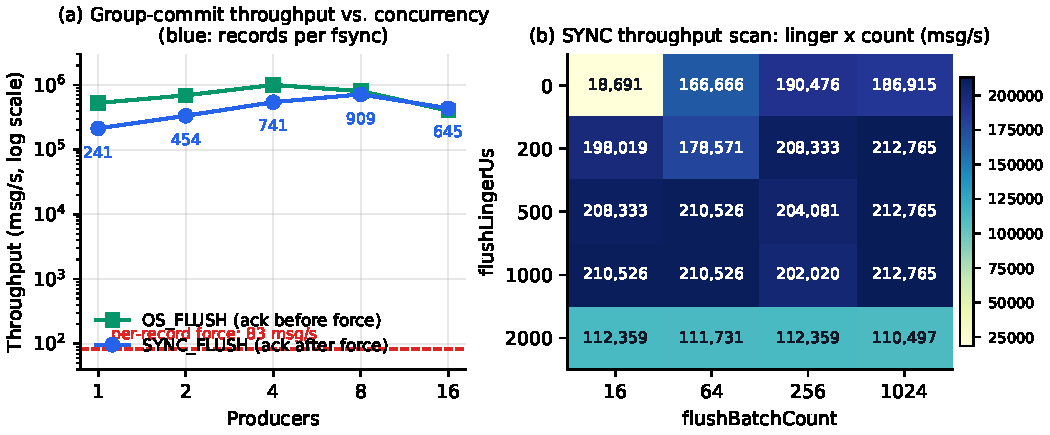
\includegraphics[width=\textwidth]{figures/fig-groupcommit.pdf}
\caption{\textbf{Group commit.} (a) SYNC-tier throughput \emph{rises}
with producer concurrency (212{,}765 $\rightarrow$ 714{,}285\,msg/s)
because the flush thread's 500\,\textmu s window aggregates more
records per \texttt{fsync} (blue labels: records per force, 241
$\rightarrow$ 909); the per-record-\texttt{fsync} baseline is 83\,msg/s,
38{,}055$\times$ below the no-force ceiling. At 8 producers the entire
cost of forcing is 11\% (714{,}285 vs.\ 800{,}000 OS-FLUSH). At 16
producers both tiers fall back---the bottleneck moves to the protocol
layer, not the disk. (b) The 5$\times$4 parameter scan that motivated
the shipped default (linger 500\,\textmu s / count 64): throughput
plateaus across the scan, collapsing only in the pathological corner
(18{,}691\,msg/s at linger 0 / count 16, i.e., near-per-record forcing)
and degrading when the window exceeds the SDK's batching period (linger
2{,}000\,\textmu s). Data: M2 \texttt{BenchV2} runs archived in
\texttt{docs/bench-v2.md}.}
\label{fig:groupcommit}
\end{figure*}

Forced durability is the classic fsync wall: with one \texttt{fsync}
per record, mini-MQ measures \textbf{83\,msg/s}, against a
no-\texttt{fsync} ceiling of 3.159\,M\,msg/s on the same engine---a
38{,}055$\times$ spread. Group commit closes almost all of it.
Figure~\ref{fig:groupcommit}(a) shows the counter-intuitive curve the
mechanism predicts and the experiment reproduces: SYNC-tier throughput
\emph{increases} with concurrency, because concurrency is precisely
what the 500\,\textmu s flush window converts into batch size---records
per \texttt{fsync} rise from 241 to 909 as producers go from 1 to 8, and
by 8 producers the full cost of forcing is \textbf{11\%} of the
no-force tier. This is the same amortization MySQL's
\texttt{ordered\_commit()} performs~\cite{mysqlbinlog,gray93tp}, with
two independent knobs---\emph{how long} to accumulate (linger) and
\emph{how much} (count)---mirroring the delay/count pair of the binlog.
Figure~\ref{fig:groupcommit}(b) is the 5$\times$4 scan that chose the
shipped defaults: the surface is a plateau (${\sim}$208--213k\,msg/s)
with exactly one collapsing corner (a window too small to aggregate,
18{,}691\,msg/s) and one degradation ridge (a window longer than the
SDK's own batching period, ${\sim}$112k). The default sits on the
plateau at the P99 knee's left edge; the choice, and the scan, are part
of the artifact.

\begin{table}[t]
\centering
\small
\begin{tabular}{llrr}
\toprule
Flush tier & Ack semantics & Acked & Lost \\
\midrule
SYNC  & after \texttt{fsync}        & 65{,}336 & \textbf{0} \\
ASYNC & before background force    & 90{,}488 & \textbf{0} \\
OS    & page cache only            & 60{,}484 & \textbf{0} \\
\bottomrule
\end{tabular}
\caption{\textbf{Crash semantics, measured with real
\texttt{SIGKILL}s.} A loaded single broker is killed at a random
moment after 10k acks, restarted through CRC recovery, and reconciled.
SYNC's zero is the tier's \emph{contract}; ASYNC's and OS's zero-loss
results are honest windows-that-were-not-hit, not proofs: ASYNC
declares a crash exposure window (unforced tail), OS declares a
power-loss window. The harness distinguishes the two statements.}
\label{tab:kill9}
\end{table}

Table~\ref{tab:kill9} prices the tiers against reality: a broker
\texttt{SIGKILL}ed mid-load, restarted, and reconciled. One subtlety
the harness enforces: an ASYNC or OS run that loses nothing must be
reported as \emph{window not hit}, not as evidence the window does not
exist. (Early in development, the shared flush counter also had a race
between concurrent appends and the in-flight force; it was replaced by
a byte-monotonic \texttt{flushedOffset} with a dedicated unit test.)

\subsection{Single broker}
\label{sec:eval-single}

\begin{figure*}[t]
\centering
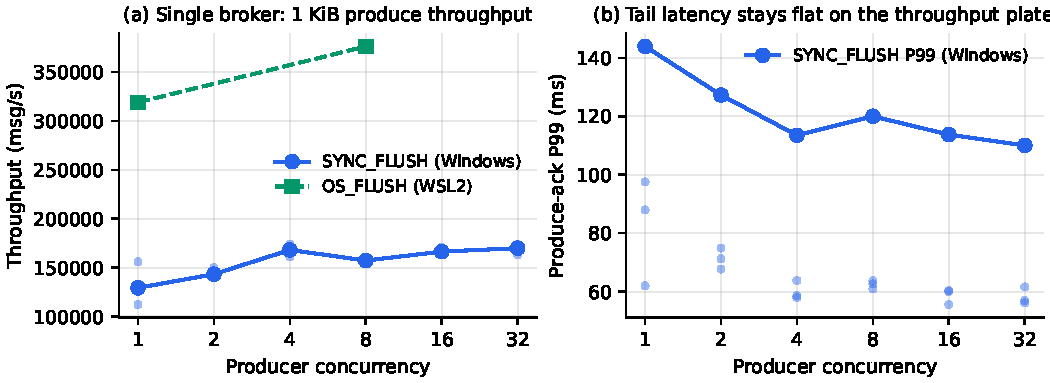
\includegraphics[width=\textwidth]{figures/fig-single.pdf}
\caption{\textbf{Single-broker produce.} Throughput (a) and produce-ack
P99 (b) across producer concurrency, full protocol stack, 1\,KiB
records, three rounds per point (dots) with medians (line). SYNC
(Windows host) plateaus at 157--170k\,msg/s with P99 flat at
${\sim}$110\,ms; OS-FLUSH (WSL2, shown for scale) reaches
376{,}350\,msg/s. Every point reconciles consumed $=$ produced. Data:
\texttt{result/m5-20261017-verified/produce.jsonl},
\texttt{result/m5-20261017-rf3-wsl/minimq-wsl-produce-os.jsonl}.}
\label{fig:single}
\end{figure*}

Figure~\ref{fig:single} shows the full protocol stack (client, Netty,
framing, dispatch, CommitLog, index) at the SYNC tier: a throughput
plateau of 157--170k\,msg/s whose P99 stays flat at ${\sim}$110\,ms,
i.e., the plateau is the honest ceiling of this stack on this host, not
a queueing collapse. On the consume side, zero-copy delivery uses
\texttt{FileRegion}/\texttt{sendfile}~\cite{bhatia04zerocopy} because
the produce path \emph{cannot} be zero-copy: it must write, index, and
CRC in user space. We report an inconvenient A/B honestly: in WSL2's
virtualized I/O stack, the sendfile path measured \emph{11.8\% slower}
than inline assembly of responses (three-round medians). The decision
record keeps the mechanism (real NICs amortize the syscall tax) while
declaring the loopback result as-is.

\subsection{Three-node cluster vs.\ same-host Kafka}
\label{sec:eval-kafka}

\begin{figure*}[t]
\centering
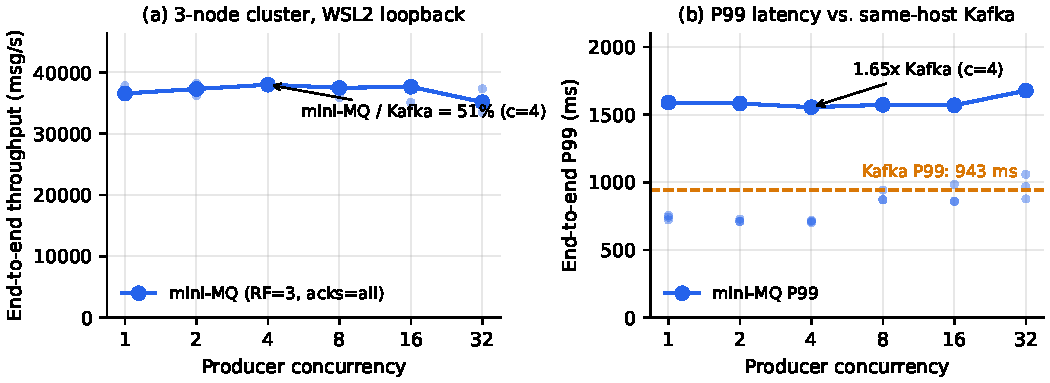
\includegraphics[width=\textwidth]{figures/fig-cluster.pdf}
\caption{\textbf{End-to-end, RF=3, \texttt{acks=all}, vs.\ Kafka 4.1.2
on the same host.} mini-MQ holds a 35--38k\,msg/s plateau from 1 to 16
producers (32 dips: the bottleneck is inside the replication loop, not
client concurrency); Kafka's median is 74{,}776\,msg/s. P99:
mini-MQ 1{,}555\,ms vs.\ Kafka 943\,ms (1.65$\times$), while P50 is at
parity (711 vs.\ 725\,ms, 0.98$\times$)---the gap is tail-shaped.
Every point reconciles; medians of three rounds with per-round scatter.
Data: \texttt{result/m5-20261017-rf3-wsl/}.}
\label{fig:cluster}
\end{figure*}

The headline comparison aligns seven dimensions (message size,
durability semantics, replication factor, \texttt{min.insync.replicas},
compression, topology, workload) and \emph{declares} the two it cannot
erase: mini-MQ's SDK batches at linger 500\,\textmu s / 64 records vs.\
Kafka's 16\,KB / 5\,ms, and rounds are 60k vs.\ 600k records (10$\times$
less JIT amortization per round for mini-MQ). Figure~\ref{fig:cluster}
shows the result: 38{,}001 vs.\ 74{,}776\,msg/s
(\textbf{51\%}), P99 1{,}555 vs.\ 943\,ms (\textbf{1.65$\times$}), P50
at parity. The flat 1-to-16-producer plateau localizes the bottleneck
inside the replication loop before any profiling is done.

\begin{table*}[t]
\centering
\small
\begin{tabular}{lp{0.34\textwidth}p{0.42\textwidth}}
\toprule
Bucket & Evidence (leader-side profiles) & Verdict \\
\midrule
\textcircled{1} Replication advances per record &
Each replicated record is one protobuf entry and one
\texttt{appendReplicated} call; fetch round-trips are linear in record
count. Kafka writes an entire produce request's records in one pass. &
Structural: the flat c=1$\rightarrow$16 curve (\S\ref{sec:eval-kafka})
is consistent with a per-record loop ceiling. \\
\textcircled{2} Protocol encoding &
Serialization frames (protobuf codec + MessageCodec) are 2.2\% of leader
CPU samples at SYNC full load. &
Real but secondary; Kafka's fixed binary format amortizes framing over
batches. \\
\textcircled{3} Storage path &
CommitLog mmap append + ConsumeQueue dispatch are 2.2\% of leader CPU
samples. &
Exculpated: both systems are page-cache sequential writes; the single
CommitLog $\approx$ one Kafka partition log. \\
\textcircled{4} Thread \& memory model &
91.6\% of leader CPU samples are G1/VM frames (6{,}177 of 6{,}742;
e.g., \texttt{OtherRegionsTable::add\_reference} 2{,}695,
\texttt{G1HotCardCache::insert} 679) at the 176k\,msg/s SYNC full-load
caliber. &
Per-record allocations on the hot path (replication read buffers,
protobuf arrays, message objects) make remembered-set maintenance the
CPU majority; Kafka's batch-oriented path allocates near-zero per record.
\emph{Caution: this bucket is a scaling wall demonstrated at the SYNC
full-load caliber; it is not a quantitative split of the 49\% RF=3
gap.} \\
\midrule
Unattributed & --- &
Declared, not hidden: same-host resource contention between the two
3-node clusters, the 10$\times$ round-length asymmetry, and two decades
of end-to-end optimization in Kafka. \\
\bottomrule
\end{tabular}
\caption{\textbf{Four-bucket attribution of the gap to Kafka.} Each
bucket carries profiled evidence; none is guessed. The share that
cannot honestly be attributed is reported as unattributed.}
\label{tab:buckets}
\end{table*}

Table~\ref{tab:buckets} is the paper's core honesty artifact: the gap
decomposed into four profiled buckets, one of which (storage) the
evidence explicitly \emph{exculpates}, and one caution note refusing to
over-read its strongest number (the 91.6\% G1 share is measured at the
SYNC single-broker full-load caliber; treating it as the RF=3 gap's
quantitative split would be dishonest, so it stays evidence of a
scaling wall, not a decomposition).

\subsection{Profiling-driven optimization}
\label{sec:eval-opt}

\begin{figure*}[t]
\centering
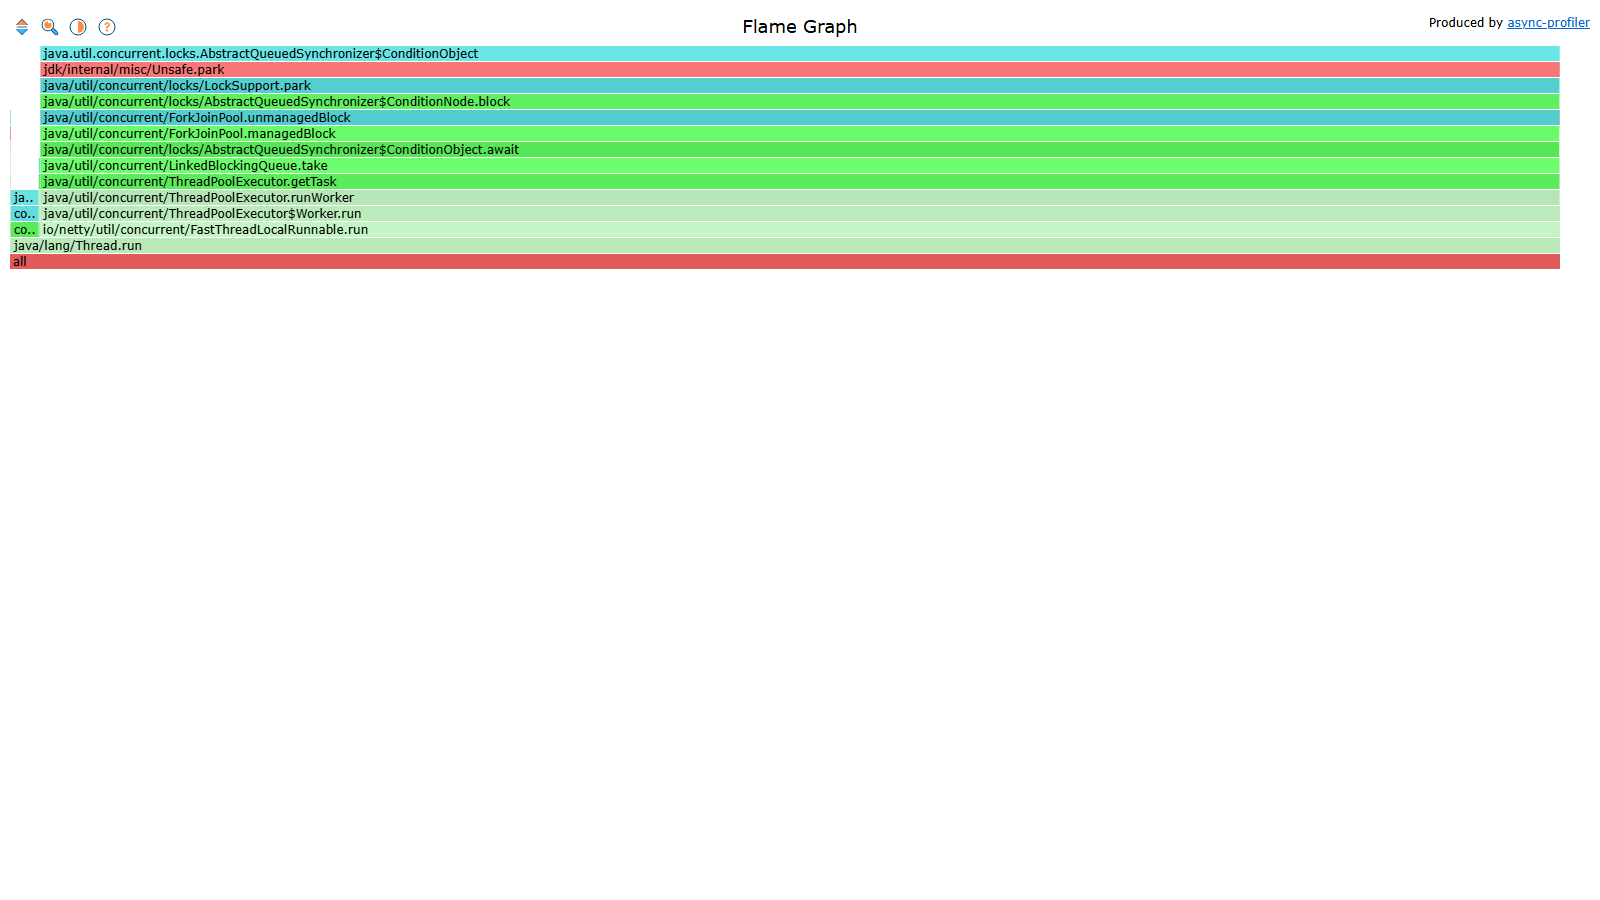
\includegraphics[width=0.49\textwidth]{figures/flame-lock-before.png}\hfill
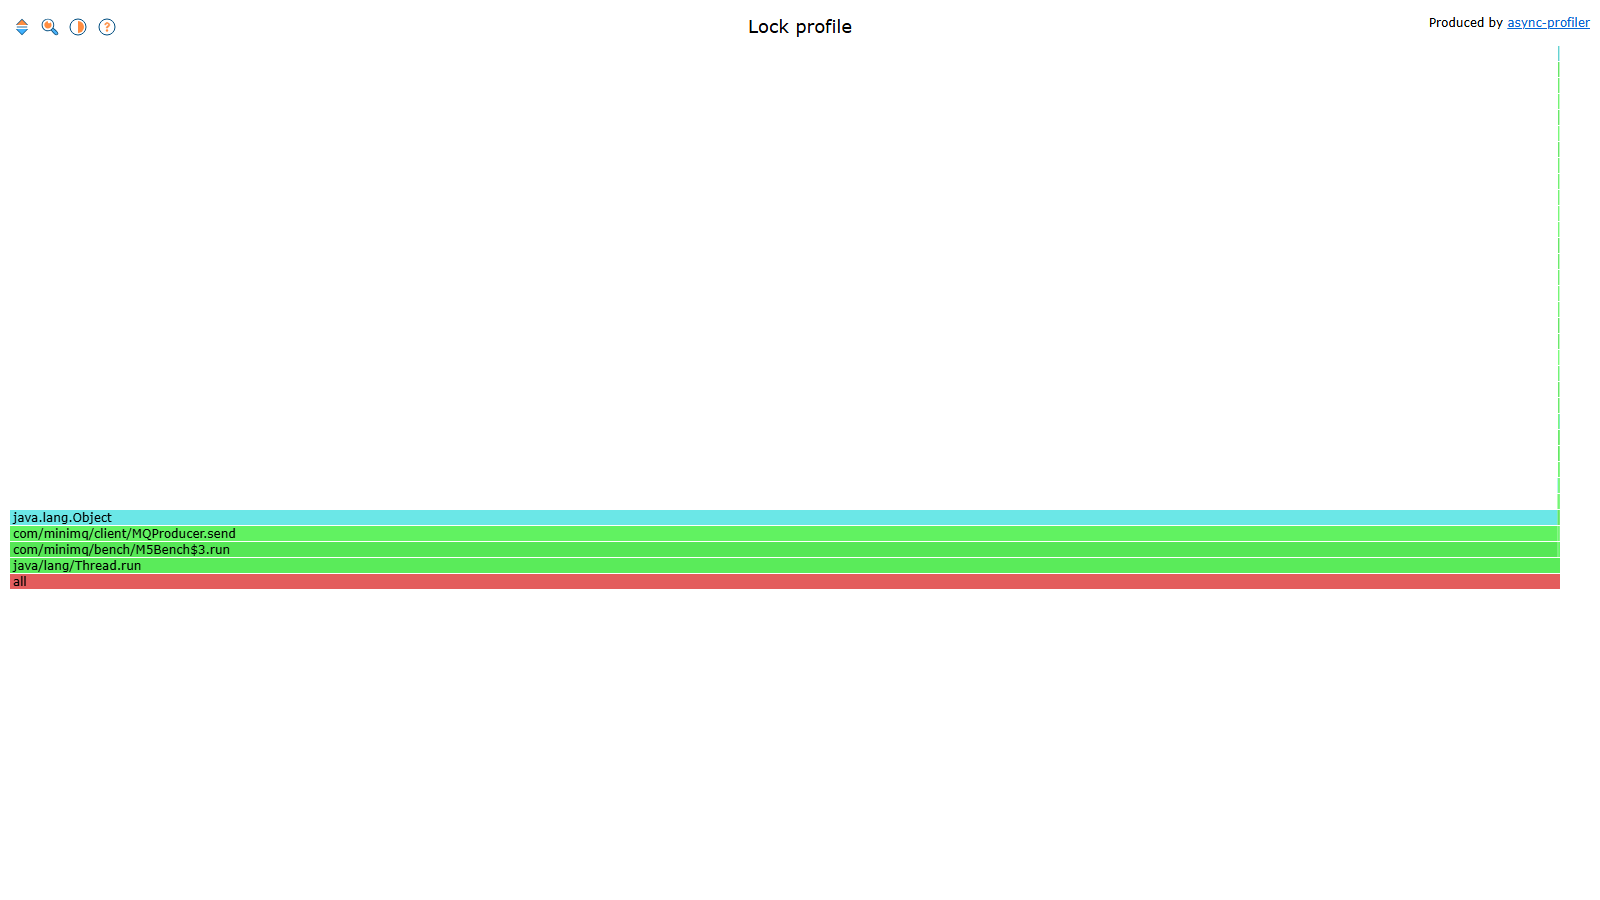
\includegraphics[width=0.49\textwidth]{figures/flame-lock-after.png}
\caption{\textbf{Lock profiles, before and after shrinking the
producer's send critical section} (8-producer SYNC full load). Left:
before---the critical section wrapped state it did not need to share,
and lock samples are 2.4\% of the profile. Right: after---the critical
section holds only the shared variable; lock samples fall to 0.3\% and
median throughput rises 171{,}865 $\rightarrow$ 177{,}691\,msg/s
(+3.4\%, medians of three rounds). Caveat declared: the two profiles
come from different toolchains (JFR before, async-profiler after), so
the comparison is of normalized shares, not raw sample counts.
Evidence: \texttt{result/flame/m5-lock-produce8c.html},
\texttt{result/m5-20261017-rf3-wsl/m5-wsl-lock-produce8c-after.html}.}
\label{fig:flame}
\end{figure*}

All three optimization stories follow the same discipline: profile
first (JFR~\cite{jep328} and async-profiler~\cite{asyncprofiler}
flame graphs are committed), change the minimum, re-measure medians of
three.

\textbf{The send-path critical section.} The lock profile showed the
producer's send critical section wrapping state it did not need to
share. Shrinking it to the single shared variable (Figure~\ref{fig:flame})
moved lock samples from 2.4\% to 0.3\% of the profile and throughput by
+3.4\%.

\textbf{Stack-rental object pools.} JFR allocation sampling pinned the
hot allocations to encode buffers and CRC32 state. The pools are
\emph{stack-rental}: a buffer is borrowed from a
\texttt{ThreadLocal}, is bound to the borrowing call stack, and has no
cross-thread escape and no explicit recycle protocol---use-after-recycle
is unrepresentable in the types. Sampled allocations fell 17.3\% on
the inline path (34.0\% where zero-copy also applies), the hot frames
vanished from the JFR top-25, and measured pool hit rates are 100\%
(17{,}920{,}418 of 17{,}920{,}450 over a 30-minute run).

\textbf{The ISR race.} Already detailed in
\S\ref{sec:chaos-bugs}: 5{,}308/60{,}000 failed writes
$\rightarrow$ 0 after the frozen-target algorithm, with the regression
test pinning the fix. We note the pattern across the three stories:
each was \emph{found} by an instrument (lock profile, allocation
profile, chaos cell) rather than by code review, and each fix is fenced
by a dedicated test.

\subsection{Stability: what only a long run finds}
\label{sec:stability}

A 30-minute rate-limited soak (10k\,msg/s, 8 producers, 512\,B records,
${\sim}$10.1\,GB across ${\sim}$38 segments, Netty leak detection at
\texttt{paranoid}) reconciled \textbf{17{,}920{,}450 acked =
17{,}920{,}450 consumed} with per-record sequence verification:
zero loss, zero duplicates, zero disorder, zero fabricated payloads.
Throughput decayed +0.2\% between the first and last five-minute
windows (i.e., none), GC trended flat (22/min falling to 6/min), leak
reports were zero.

The soak's unique catch: at minute 7, consumption halved, then
collapsed, while GC spiked to 268 collections/min and CPU burned in
\texttt{ConsumeQueue} dispatch. The cause was a
\texttt{int}-multiplication overflow in segment lookup
(\texttt{idx * segmentSize}) exactly at the 2\,GiB boundary (segment
8's base $=2^{31}$): the cursor silently reset and dispatch re-read
the segment head in an infinite loop, re-CRCing the same 512 records
${\sim}$767$\times$ each. Every other test in the suite writes less
than 2\,GB---\emph{only} the soak crossed the boundary. The fix (range
comparison in \texttt{long}) is fenced by a regression test that
hand-builds a sparse $3\times$1\,GiB segment chain so the boundary is
testable without writing 2\,GB. The lesson generalizes: byte-offset
arithmetic belongs in \texttt{long} everywhere, and long-horizon runs
are the only tests that reach quantity-becomes-quality failure modes.

%-------------------------------------------------------------------------------
\section{Limits, Declared}
%-------------------------------------------------------------------------------
We state what mini-MQ deliberately is not, because a system's claims
are only as good as its stated boundaries~\cite{nygard11adr}:

\begin{itemize}
\item \textbf{No cross-session exactly-once.} Dedup is
  leader-session-scoped; a retry that lands on a different leader
  appends again. Final arbitration is consumer-side idempotency by
  \texttt{seq\_key}.
\item \textbf{One write stream per broker.} All topics share a single
  CommitLog, so write parallelism is bounded by one sequential file.
  The decision is recorded with its invalidation boundary: it flips
  the day single-file sequential writes become the bottleneck.
\item \textbf{No consumer-group rebalance} (subscriptions are static)
  \textbf{and no security layer} (no TLS, no authentication, no ACLs).
\item \textbf{Scale evidence is three nodes on one host (loopback).} No
  claim is made about 30 nodes, cross-DC replication, or cloud
  topologies.
\item \textbf{Benchmark numbers are Linux-side (WSL2).} The Windows
  host runs the tests, but NTFS-native mmap semantics are not a
  maintained benchmark caliber; and no \texttt{docker-compose} is
  shipped, because the development machine's Docker daemon could not
  validate one---an untested one-click file would break the ten-minute
  promise it makes.
\item \textbf{A declared share of the Kafka gap is unattributed}
  (Table~\ref{tab:buckets}), and honest attribution is worth more
  than a fully-explained fiction.
\end{itemize}

%-------------------------------------------------------------------------------
\section{Related Work}
%-------------------------------------------------------------------------------------------
\textbf{Production message queues.} Kafka~\cite{kreps11kafka,kafkadocs}
established the partitioned-log model with pull replication, leader
epochs, and ISR semantics; RocketMQ~\cite{rocketmqdocs} the single
CommitLog with replayed consume queues; Pulsar~\cite{pulsardocs}
segmented ledgers and compute-storage separation. mini-MQ borrows one
gene from each and, uniquely among the three, is small enough to read
in an afternoon. \textbf{Consensus and control planes.} Raft's
understandability argument~\cite{ongaro14raft} motivated our election
kernel; KRaft~\cite{kip500} validated separating a Raft-style metadata
plane from fetch-based data replication, a split mini-MQ shares.
\textbf{Educational systems.} xv6~\cite{xv6} plays the same role for
operating systems that mini-MQ aims to play for messaging: real
mechanisms, executable size. \textbf{Group commit} is classical
transaction-processing wisdom~\cite{gray93tp}, productionized in
MySQL's \texttt{ordered\_commit()}~\cite{mysqlbinlog}. \textbf{Chaos
engineering.} The Simian Army~\cite{netflix11simian} and the chaos
discipline~\cite{basiri16chaos} injected faults in production; mini-MQ
contributes \emph{deterministic, moment-named} injection at bare-JVM
scale, where container-era tooling does not reach.

%-------------------------------------------------------------------------------
\section{Conclusion}
%-------------------------------------------------------------------------------
mini-MQ shows that the load-bearing mechanisms of industrial message
queues---sequential-log storage with CRC recovery, two-parameter group
commit, pull replication with epoch arbitration and watermarks, a Raft
election kernel, deduplication and dead letters---can be built
honestly at learning scale: with faults injected at named moments, with
invariants hard-asserted per cell, with optimizations driven by
committed flame graphs, and with the industry comparison reported as a
loss (51\%, 1.65$\times$) whose anatomy is profiled bucket by bucket
and whose unexplained remainder is declared rather than decorated. We
believe the reusable contribution is the \emph{caliber}: a recipe for
what a small system must measure, assert, and admit in order for its
green lights to mean something.

%-------------------------------------------------------------------------------
\section*{Availability}
\label{sec:availability}
%-------------------------------------------------------------------------------
mini-MQ is open source under the MIT license:
\begin{center}
\url{https://github.com/Xstly1014/mini-MQ}
\end{center}
One command builds it, boots a three-node cluster, reconciles a
10{,}000-message smoke run (asserting \texttt{lost=0 dup=0}), and tears
it down:
\begin{center}
\texttt{bash bench/quickstart.sh}
\end{center}
Every performance number in this paper regenerates from committed
evidence files: \texttt{paper/make-figures.py} rebuilds all figures
from the JSONL artifacts in \texttt{result/}, and the benchmark scripts
in \texttt{bench/} rerun every experiment end to end. The 209-test
regression suite, including the 12-cell chaos matrix, runs with
\texttt{mvn clean test}. Eight architecture decision records
(\texttt{docs/adr/}) document each major choice with its rejected
alternatives.

%-------------------------------------------------------------------------------
\bibliographystyle{plain}
\bibliography{refs}

%%%%%%%%%%%%%%%%%%%%%%%%%%%%%%%%%%%%%%%%%%%%%%%%%%%%%%%%%%%%%%%%%%%%%%%%%%%%%%%%
\end{document}
%%%%%%%%%%%%%%%%%%%%%%%%%%%%%%%%%%%%%%%%%%%%%%%%%%%%%%%%%%%%%%%%%%%%%%%%%%%%%%%%
